This is about the Sharp Particulate Sensor results.

One Sharp optical particulate sensor was tested against the EPA black carbon reference.  It was 1 month old at the time of installation, and ran for 59 days (from 4/15 - 6/13 2016) with two ~40 minute service interruptions.  This test gave 1,431 samples of hour resolution data.


\subsection{Pre-processing}

Talk about process for taking raw aux/working electrodes and making the basic calibration data.
10am reading of EPA sensor is recorded on filter paper from 10a-10:50a, then measured with Beta Attenuation from 10:50-11a.  Thus, we averaged the 50 minute readings starting on the hour and threw away the last ten minutes.  Added some feature averaging on the 6hr , 12hr, day scale.

\begin{figure}[htb]
 	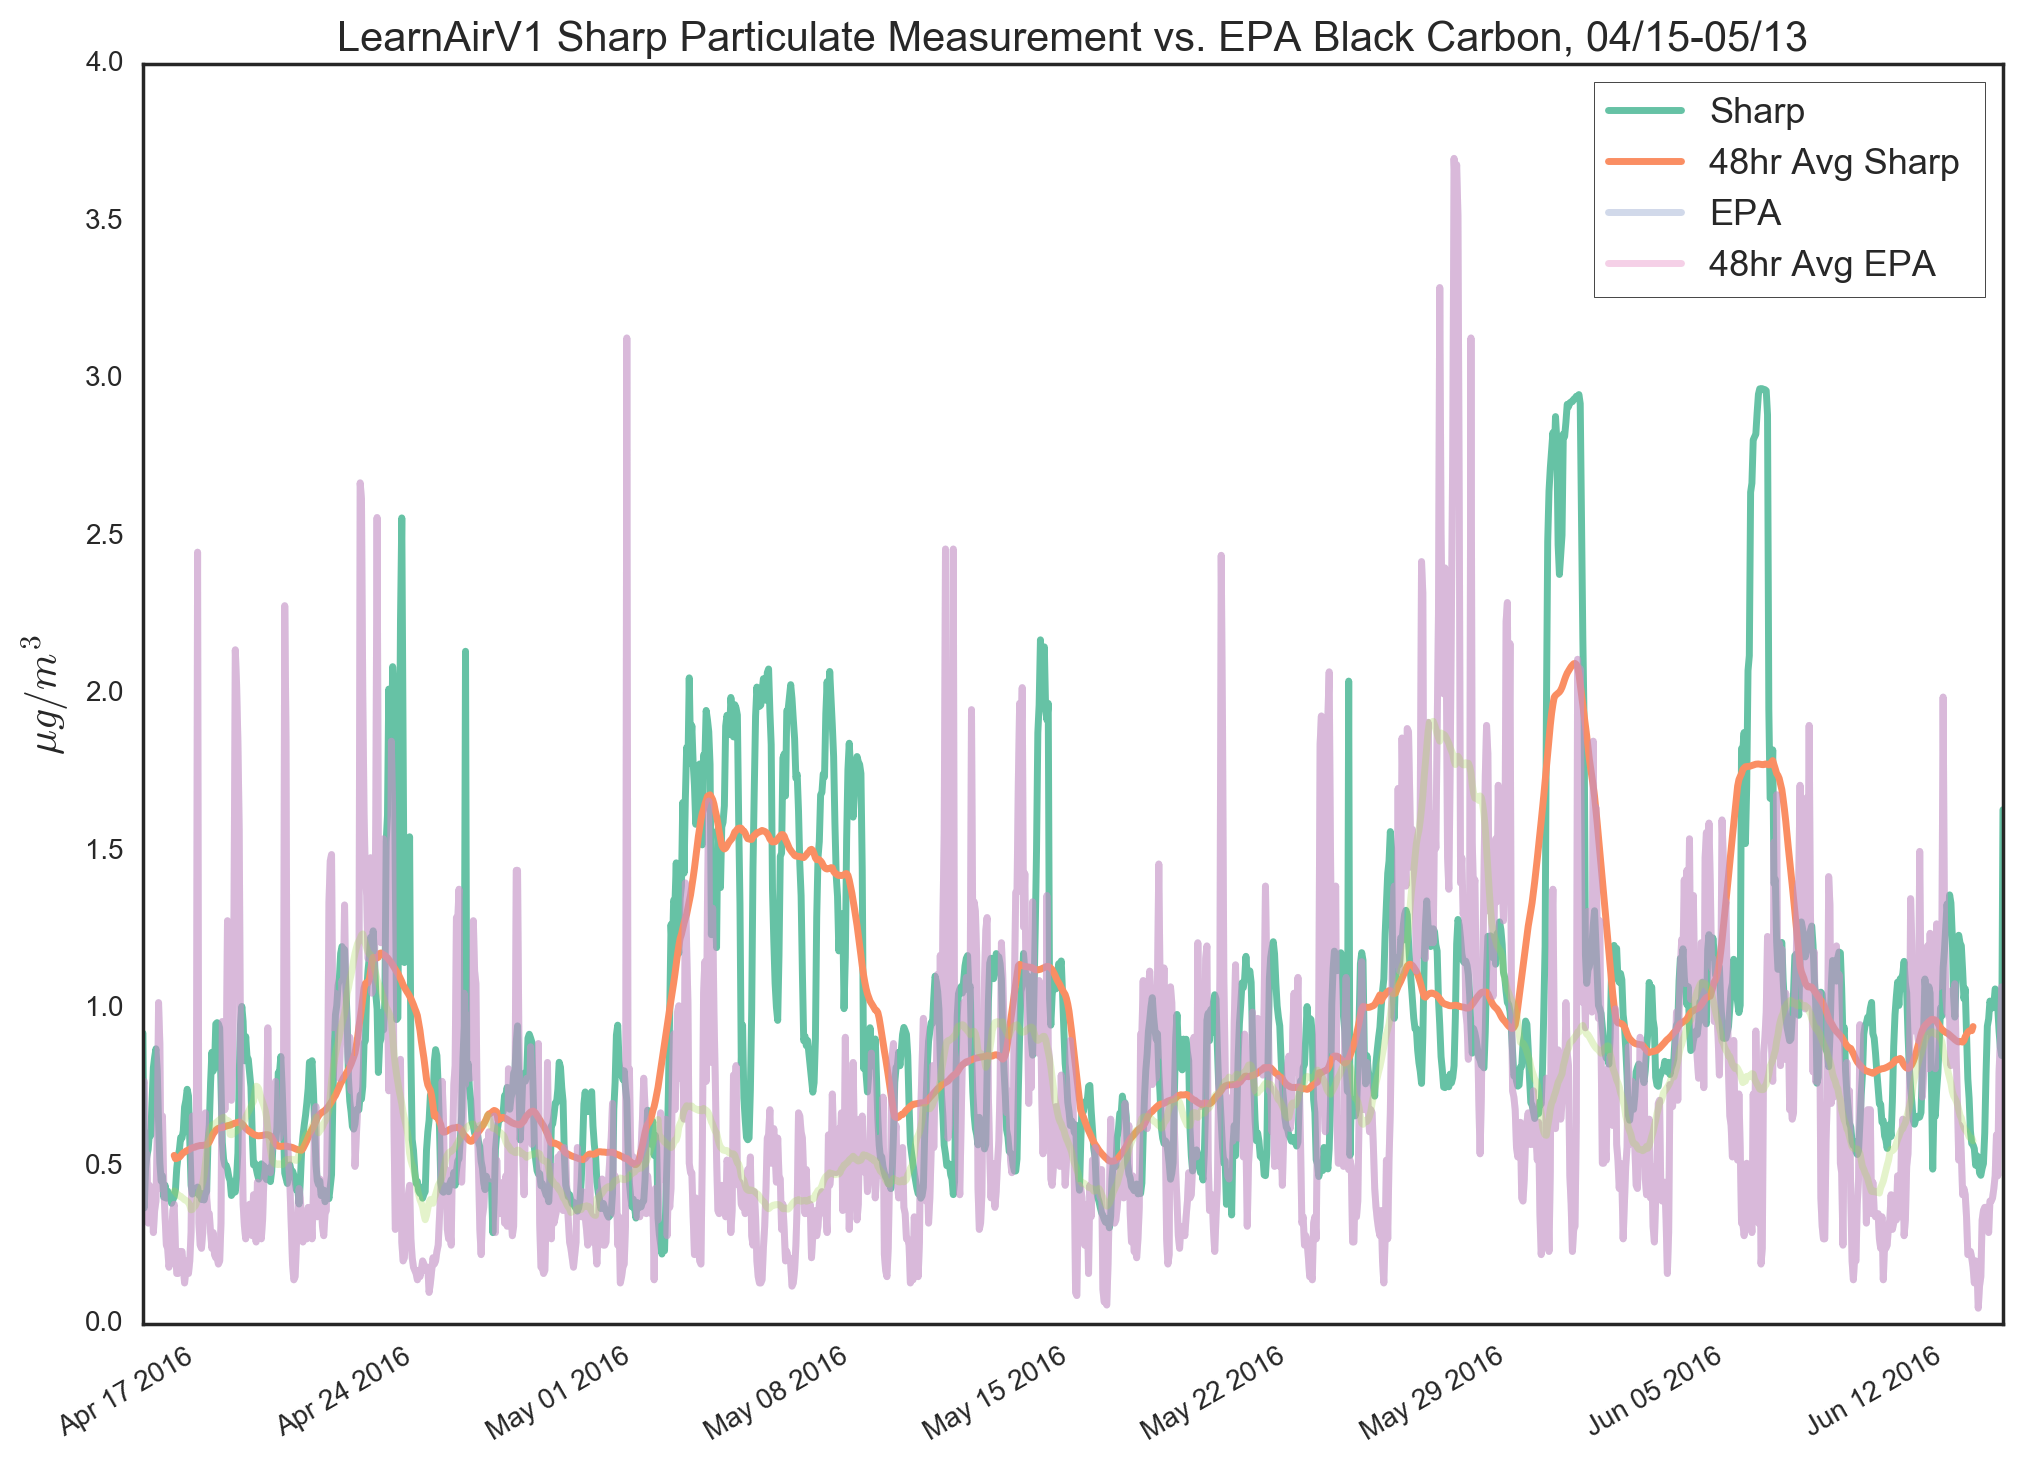
\includegraphics[width=\textwidth]{figs/sharp_raw}               
 	 \caption{Sharp Raw Particulate Data}
  	\label{fig:sharp_raw}
\end{figure}


\begin{figure}[htb]
 	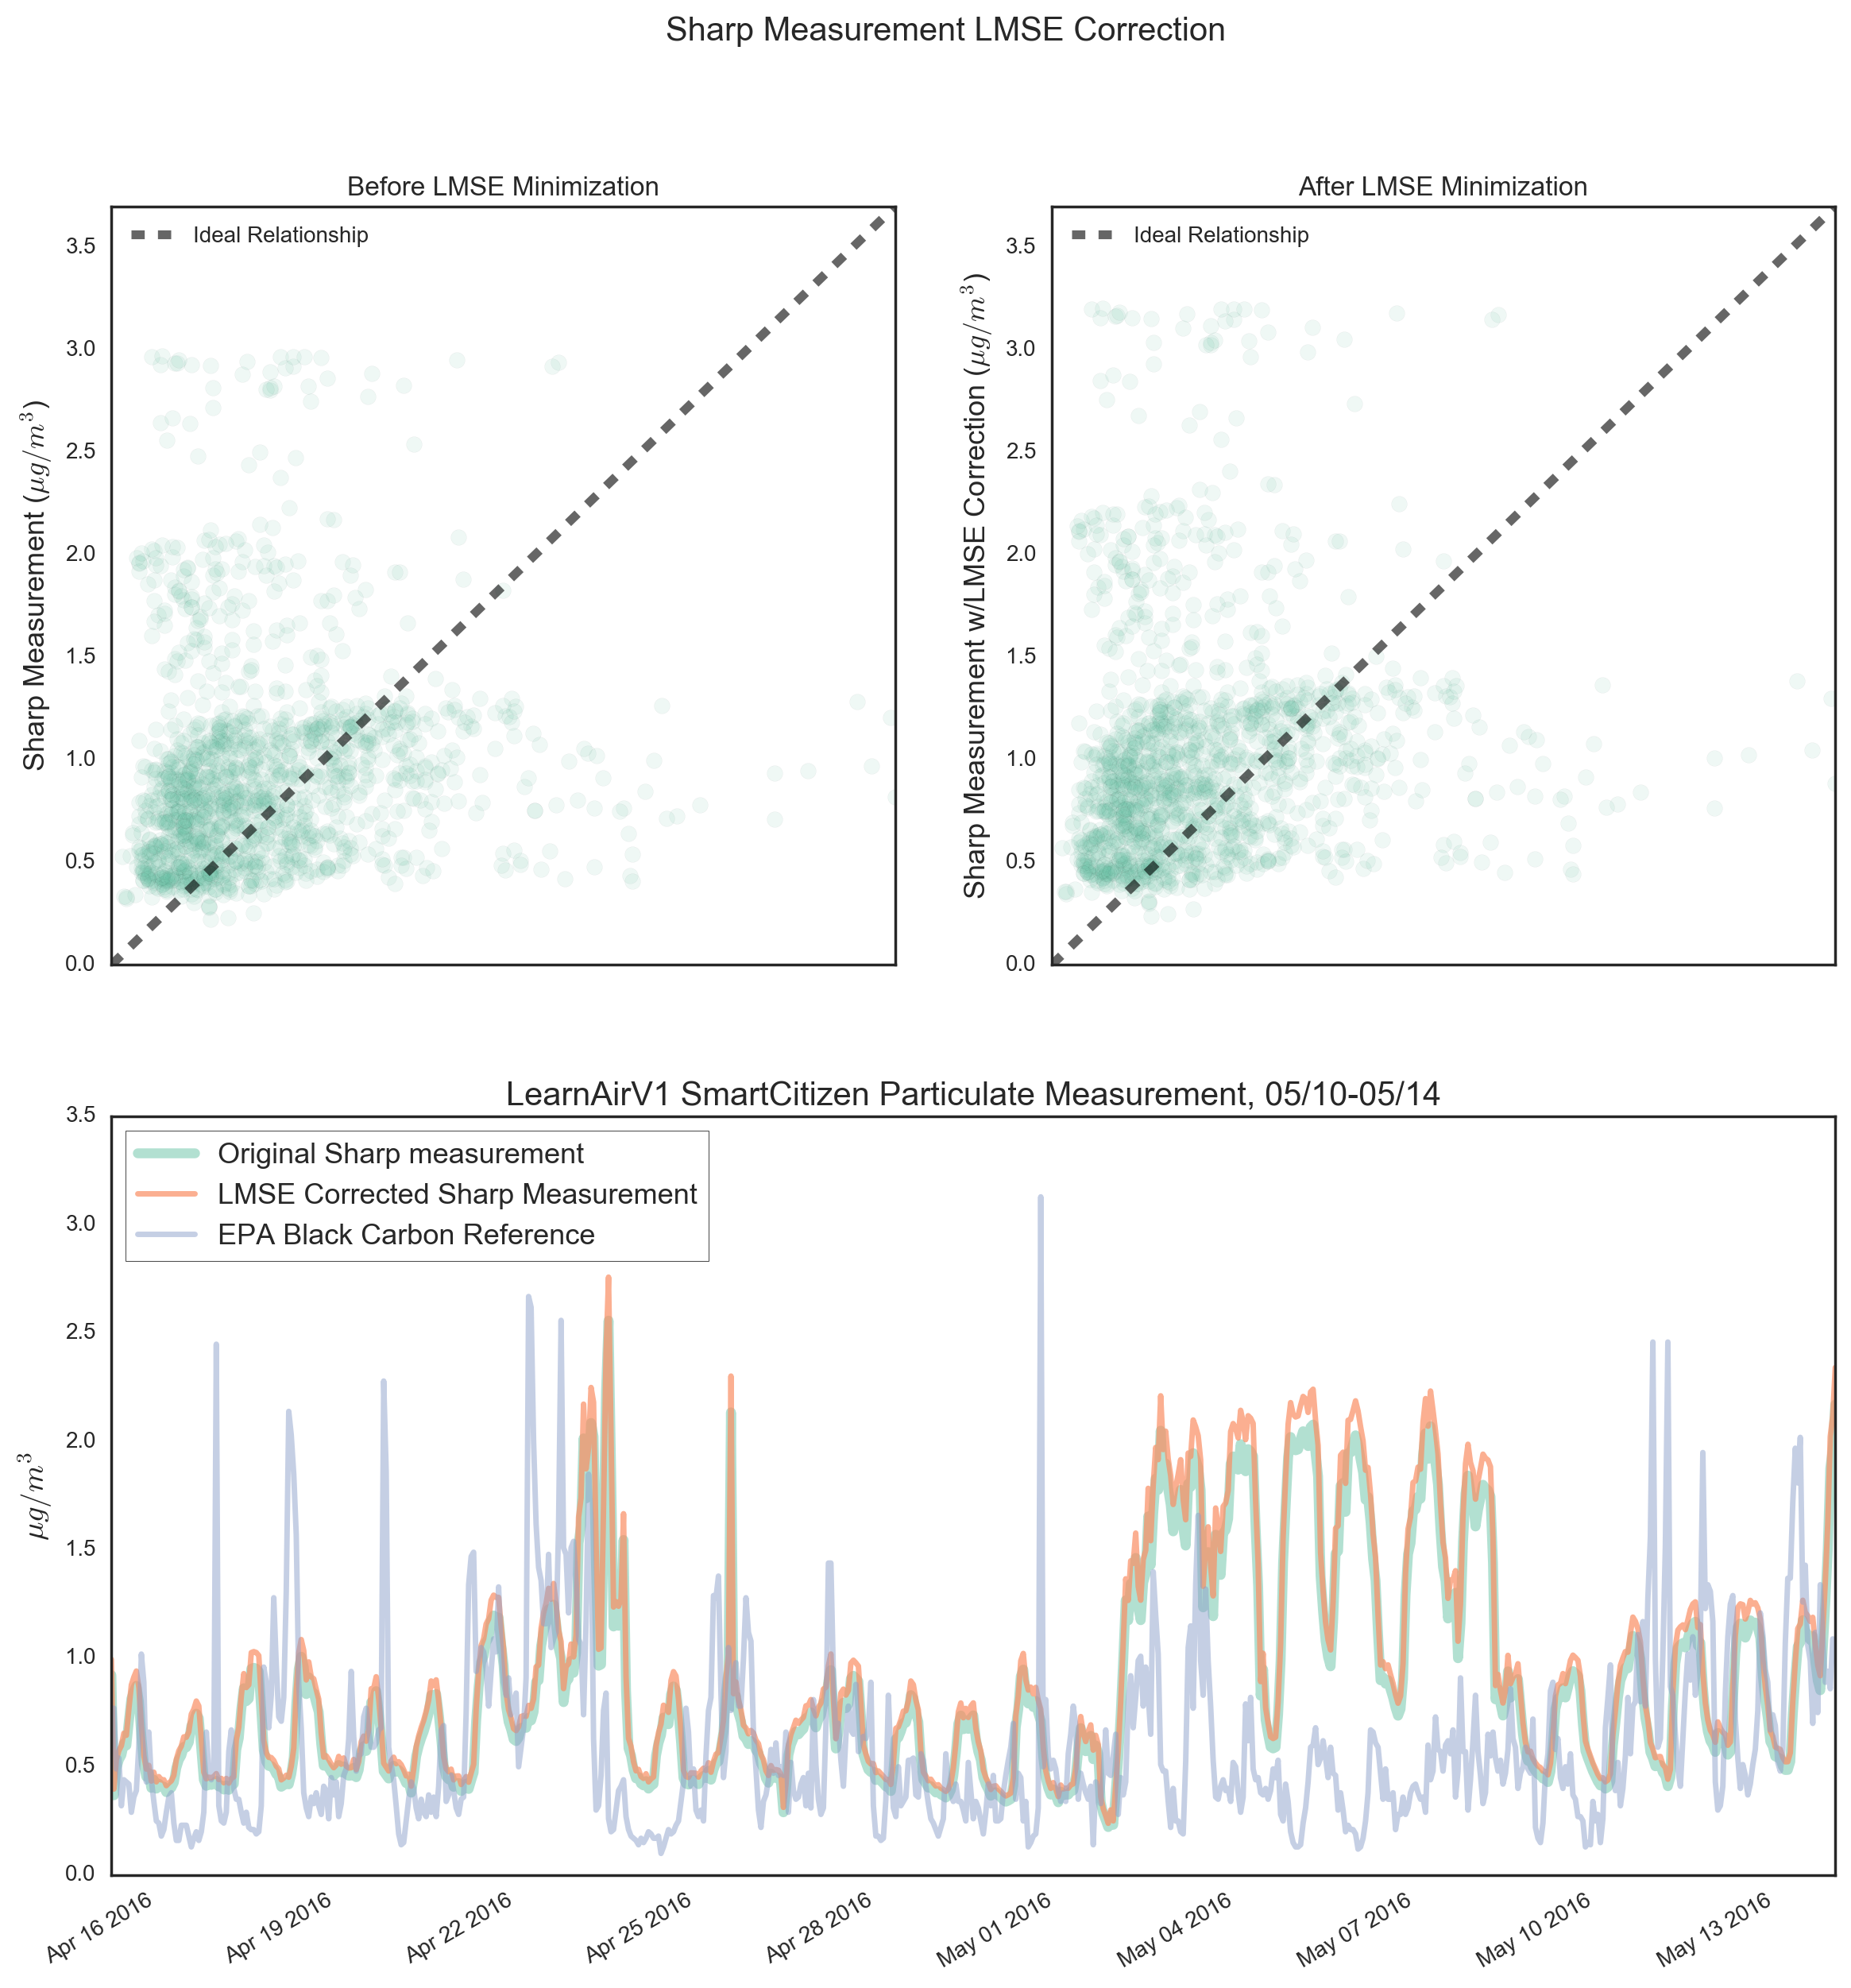
\includegraphics[width=\textwidth]{figs/sharpDust_lmse}               
 	 \caption{Sharp Particulate LMSE Calibration}
  	\label{fig:sharpDust_lmse}
\end{figure}

\begin{figure}[htb]
 	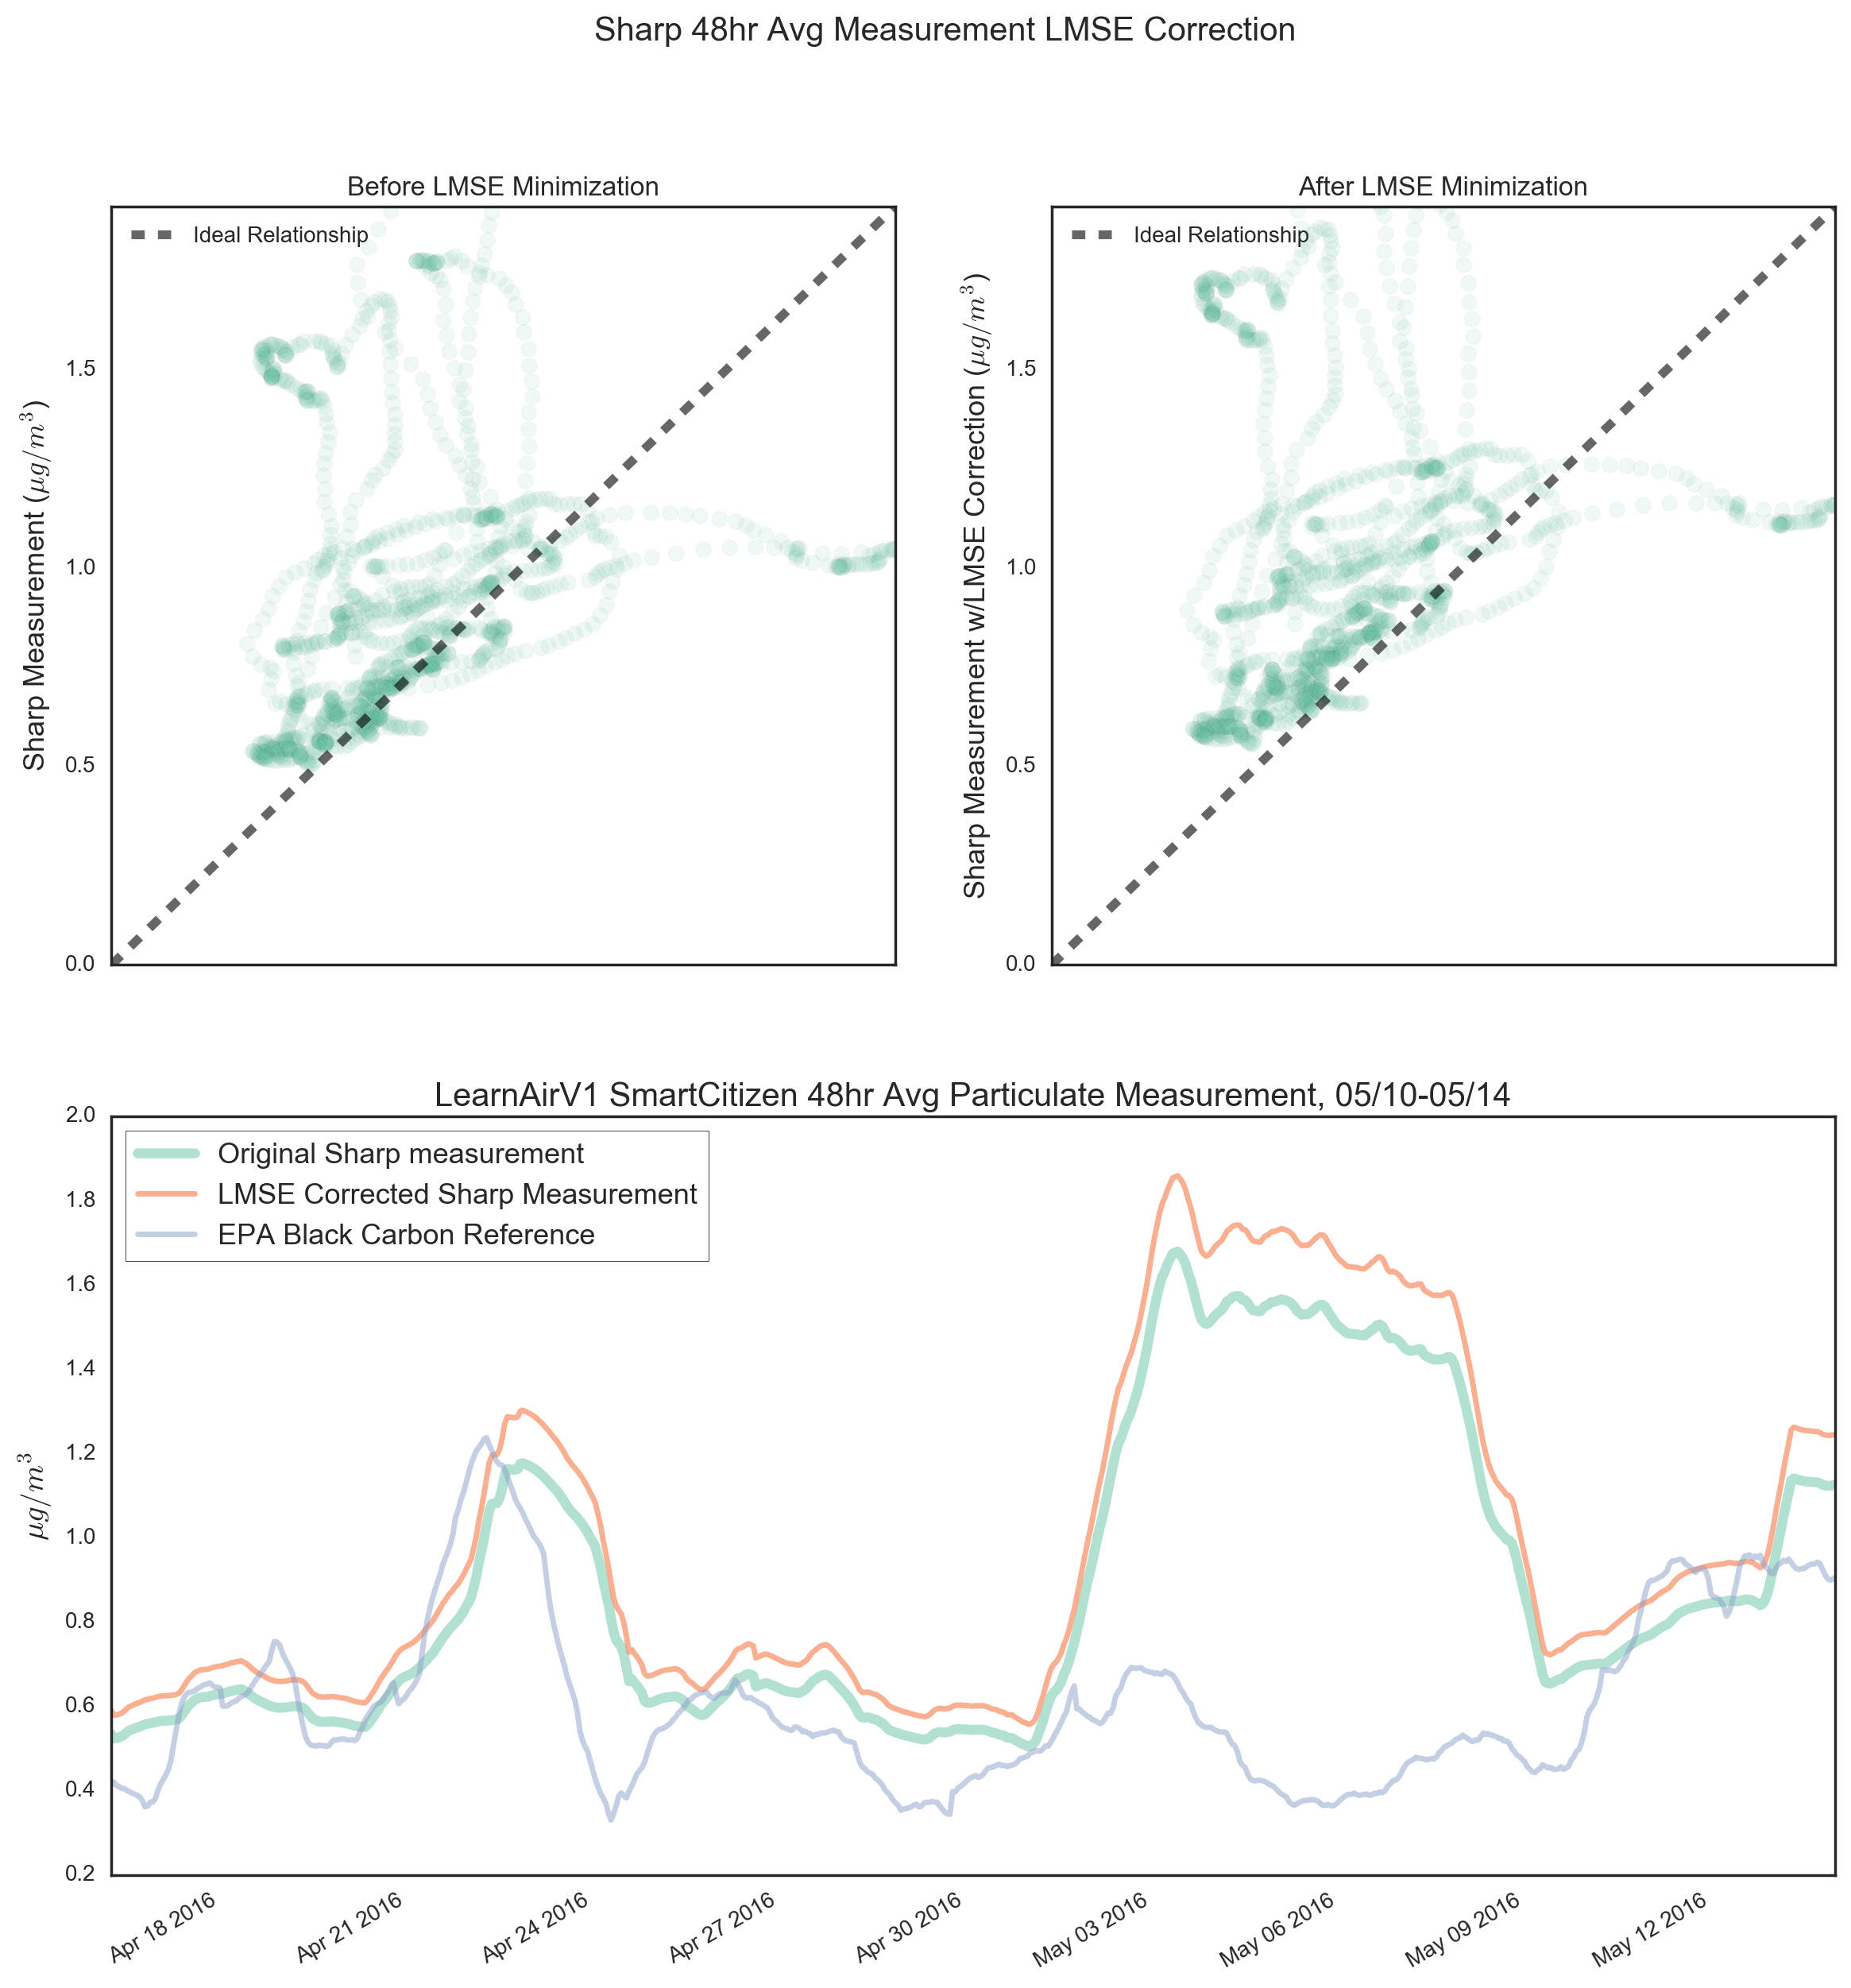
\includegraphics[width=\textwidth]{figs/sharpDust_avg_48_lmse}               
 	 \caption{2 day Average Sharp Particulate LMSE Calibration}
  	\label{fig:sharpDust_avg_48_lmse}
\end{figure}







\subsection{Machine Learning}


\begin{figure}[htb]
 	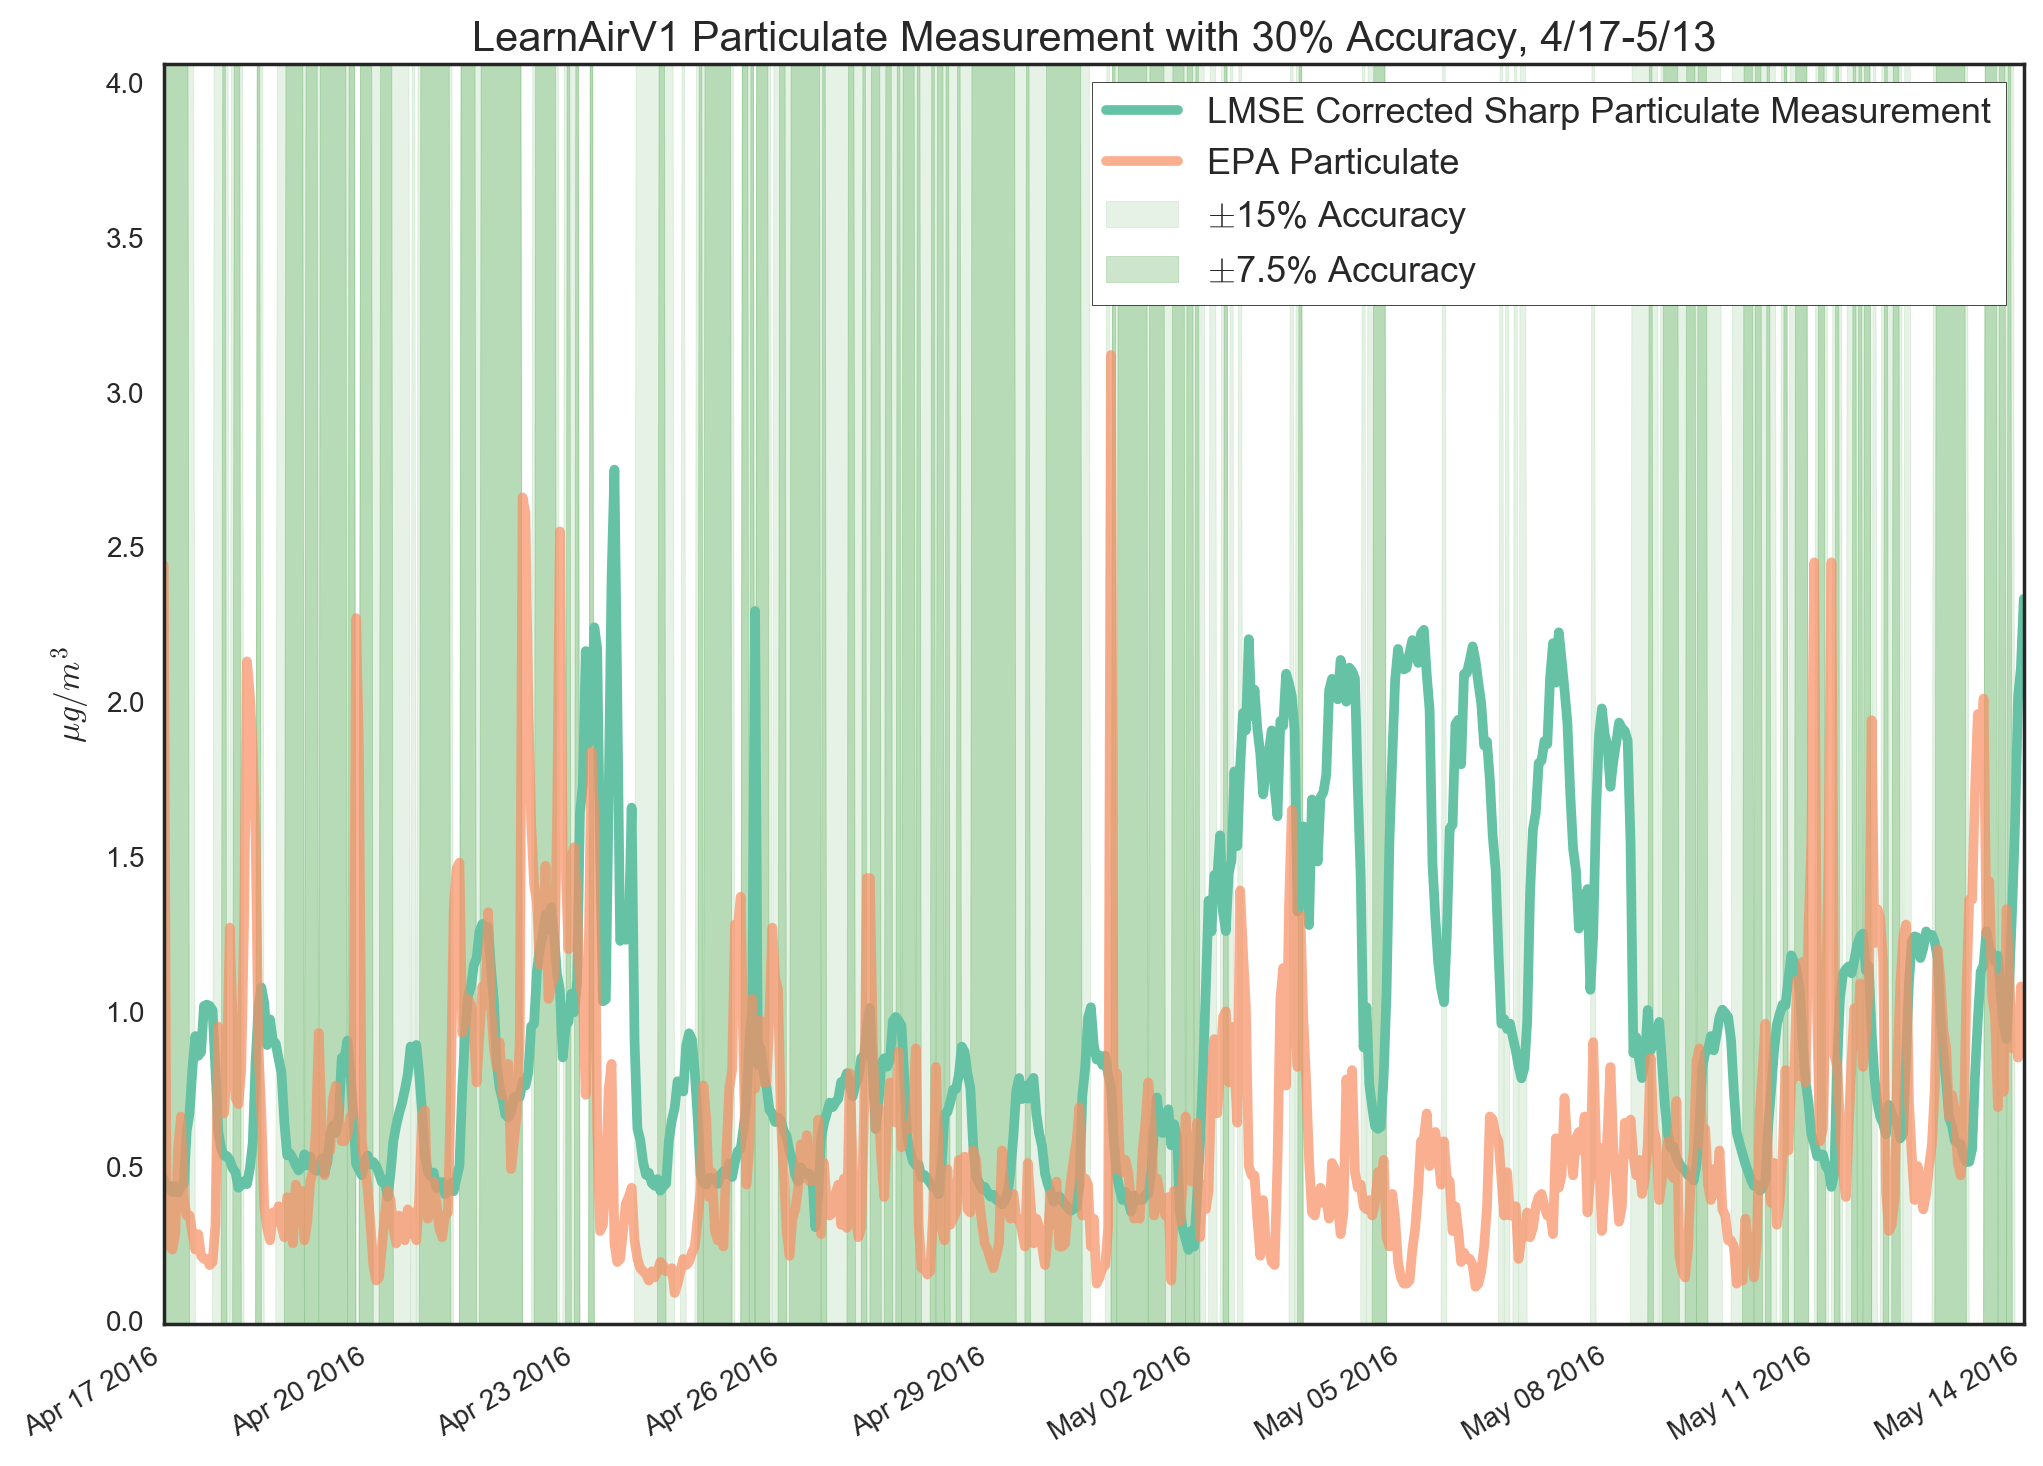
\includegraphics[width=\textwidth]{figs/sharpDust_with_accuracy_zoomed}               
 	 \caption{Sharp Particulate with 30\% Accuracy Threshold}
  	\label{fig:sharpDust_with_accuracy_zoomed}
\end{figure}




parameters = {'C':[0.001, 0.01, 0.1, 1, 10, 100, 1000], 'penalty':('L1', 'L2') }, true 5 fold validation

===== best ROC\_AUC score 0.868191734814

===== best params {'penalty': 'L1', 'C': 1}



\begin{table}[H]
\centering
\begin{tabular}{|c|c|c|c|c|}
\toprule
\multicolumn{5}{|c|}{Error Rates for CO Sensor #1 with Logistic Regression} \\
&\multicolumn{2}{|c|}{all features} & \multicolumn{2}{|c|}{top 15 features} \\
&shuffled & chunked & shuffled & chunked \\
avg & 0.17 & 0.22 & 0.22 & 0.25 \\
min & 0.14 & 0.18 & 0.20 & 0.14 \\
max & 0.20 & 0.29 & 0.24 & 0.36 \\
\bottomrule
\end{tabular}
\label{tab:as1_co_error_rates}
\caption{Error Rates for Predicting Sharp Accuracy with Logistic Regression}
\end{table}



\begin{table}[H]
\centering
\offinterlineskip
\hspace*{-5cm}\raisebox{-3.5cm}[0pt][0pt]{\rotatebox[origin=c]{90}{\parbox[c][0pt][c]{3cm}{\textbf{Actual Values}\\[20pt]}}}\par
\hspace*{1cm}\MyHBox[\dimexpr5.1cm+6\fboxsep\relax]{Predicted Values}\par
\hspace*{1cm}\MyHBox{0}\MyHBox{1}\par
\MyTBox{0}{58.0}{35.2}
\MyTBox{1}{14.0}{179.0}
}
\label{tab:as1_co_confusion}
\caption{Average Sharp Particulate Confusion Matrix w/Shuffled K-Fold}
\end{table}


\begin{figure}[htb]
 	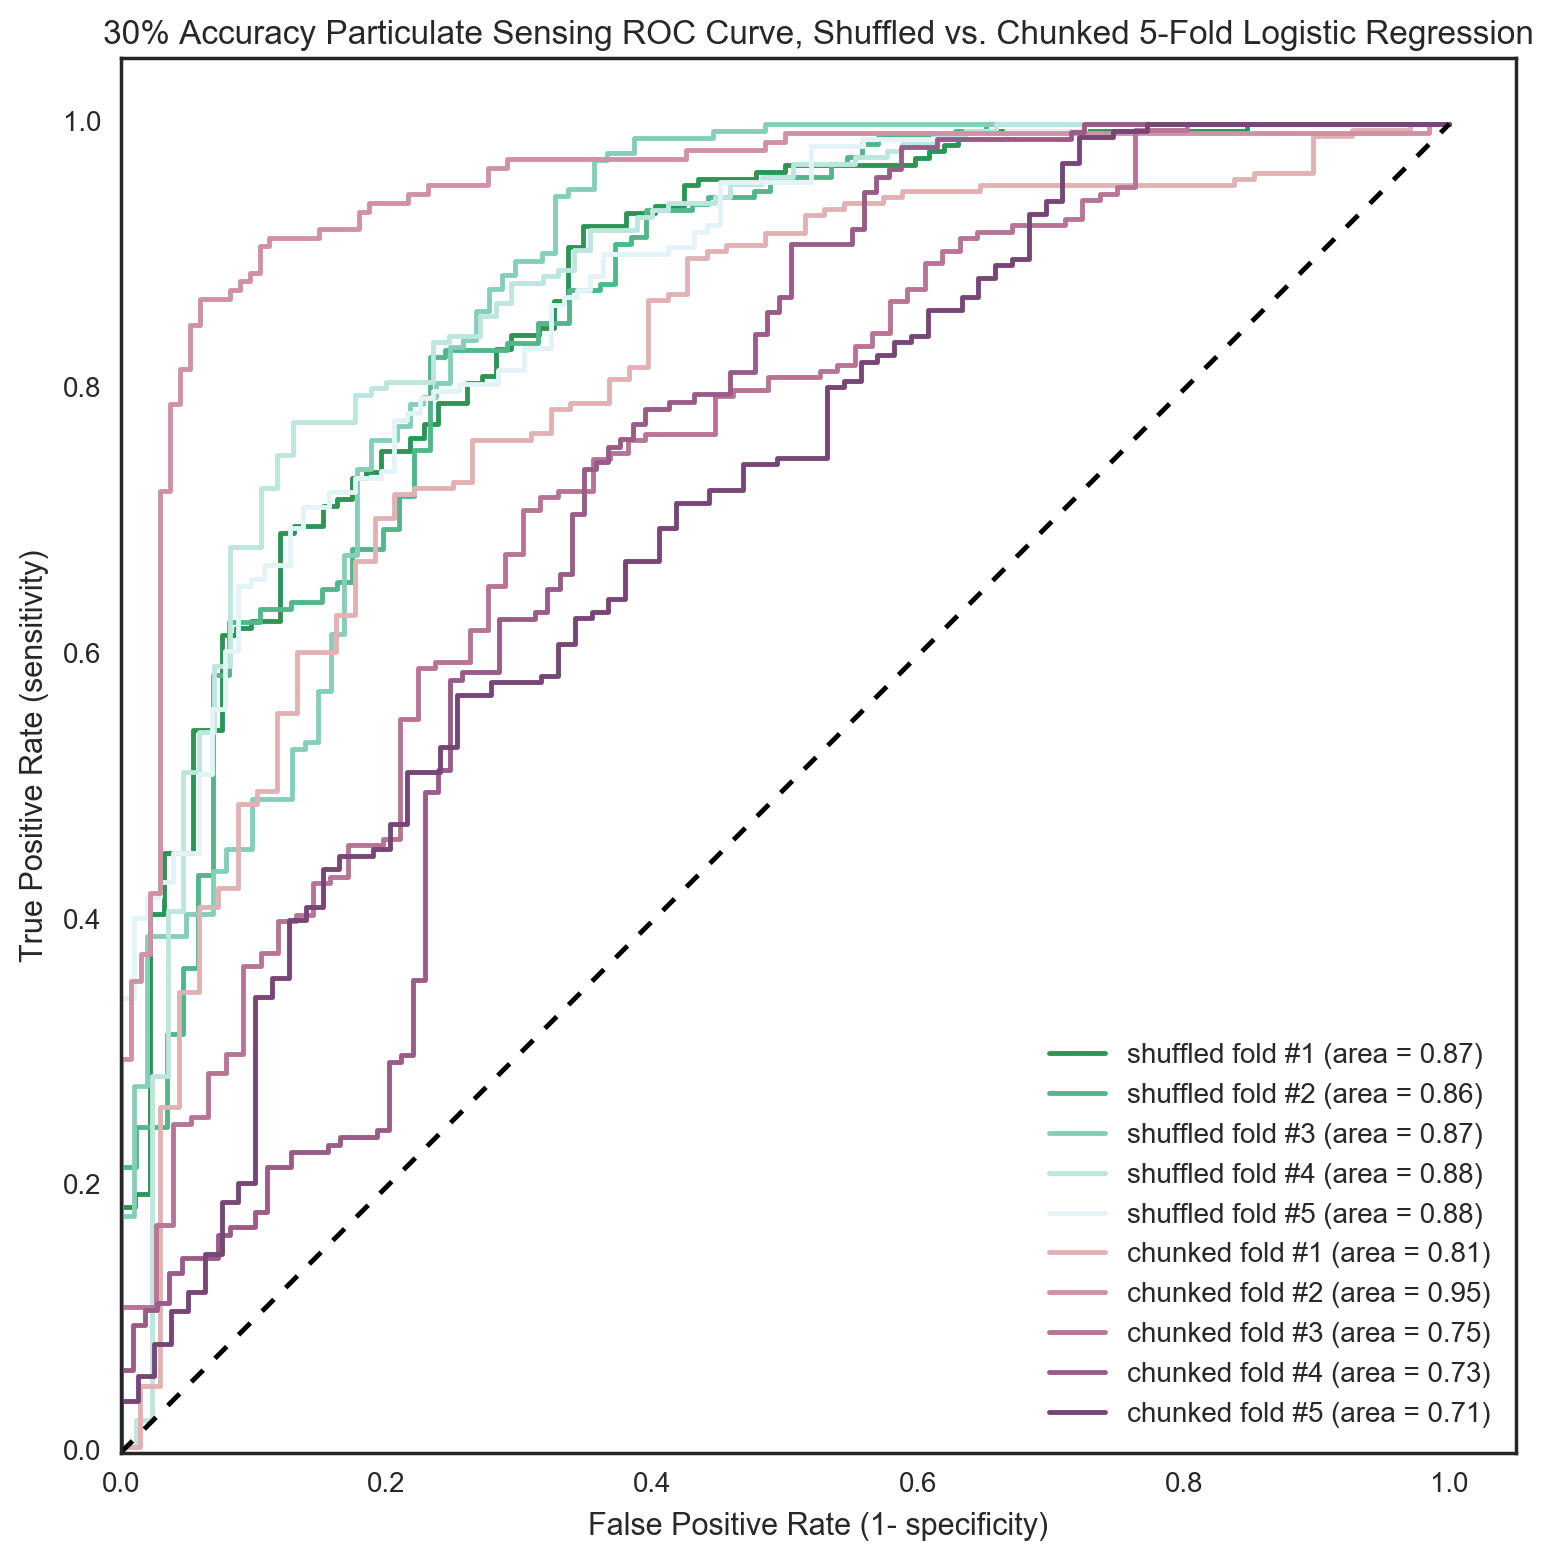
\includegraphics[width=\textwidth]{figs/sharp_goals_30_roc}               
 	 \caption{Sharp Particulate ROC Curve}
  	\label{fig:sharp_30_roc}
\end{figure}


here's text referencing the (Table \ref{tab:sharp_randomforest_features}).

\begin{table}[H]
\centering
\begin{tabular}{lllllllll}
\\
\\
\toprule
Feature & Importance \\
\midrule
 scaled\_sharpDust &  0.039935725943 \\
 avg\_12\_scaled\_sharpDust &  0.0390147943972 \\
 sharpDust &  0.0390147211728 \\
 lmse\_scaled\_sharpDust &  0.0381632767126 \\
 avg\_48\_scaled\_sharpDust &  0.0225005941711 \\
 lmse\_avg\_48\_scaled_sharpDust &  0.0207695248823 \\
 sck\_humidity &  0.0163292725576 \\
 Humidity ( % RAW) &  0.0162400825573 \\
 no2 &  0.0149758603207 \\
 daily\_avg\_sck\_humidity &  0.0138699992039 \\
 daily\_avg\_forecastio\_humidity &  0.0132135840929 \\
 humidity\_box\_differential &  0.0119641893085 \\
 co &  0.0118968560369 \\
 sck\_humidity\_saturated &  0.0103888721788 \\
 avg\_60\_forecastio\_humidity &  0.0102980544091 \\
\bottomrule
\end{tabular}
\label{tab:sharp_randomforest_features}
\caption{Top 15 Features from Random Forest for Sharp Sensor, used in Pruned Logistic Regression}
\end{table}



\begin{figure}[htb]
 	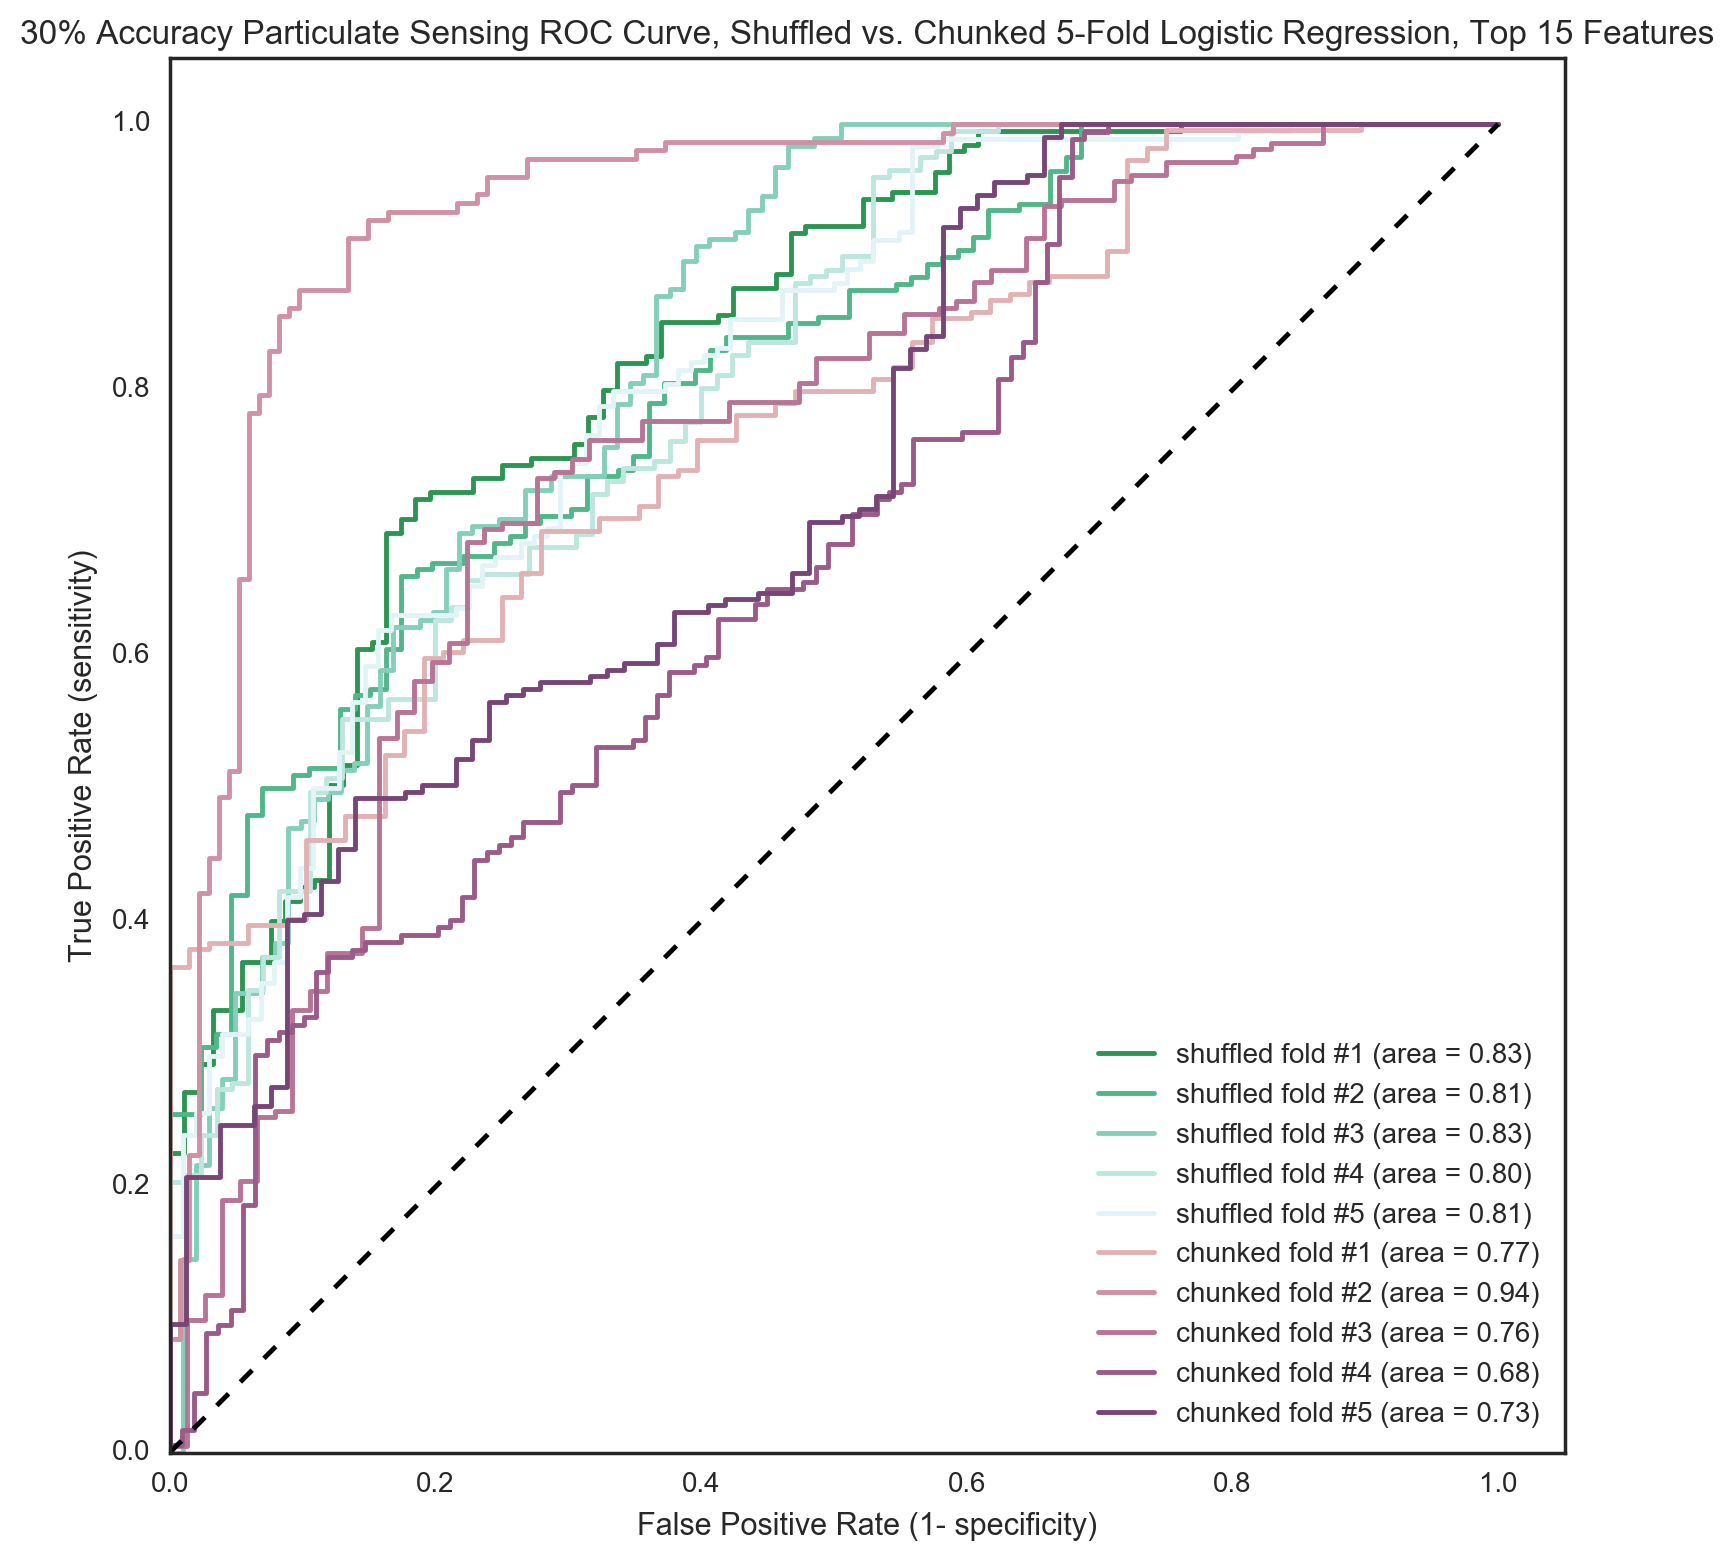
\includegraphics[width=\textwidth]{figs/sharp_goals_30_roc_pruned_features}               
 	 \caption{Sharp Particulate ROC Using Top 15 Features}
  	\label{fig:sharp_30_roc_pruned_features}
\end{figure}

\begin{figure}[htb]
 	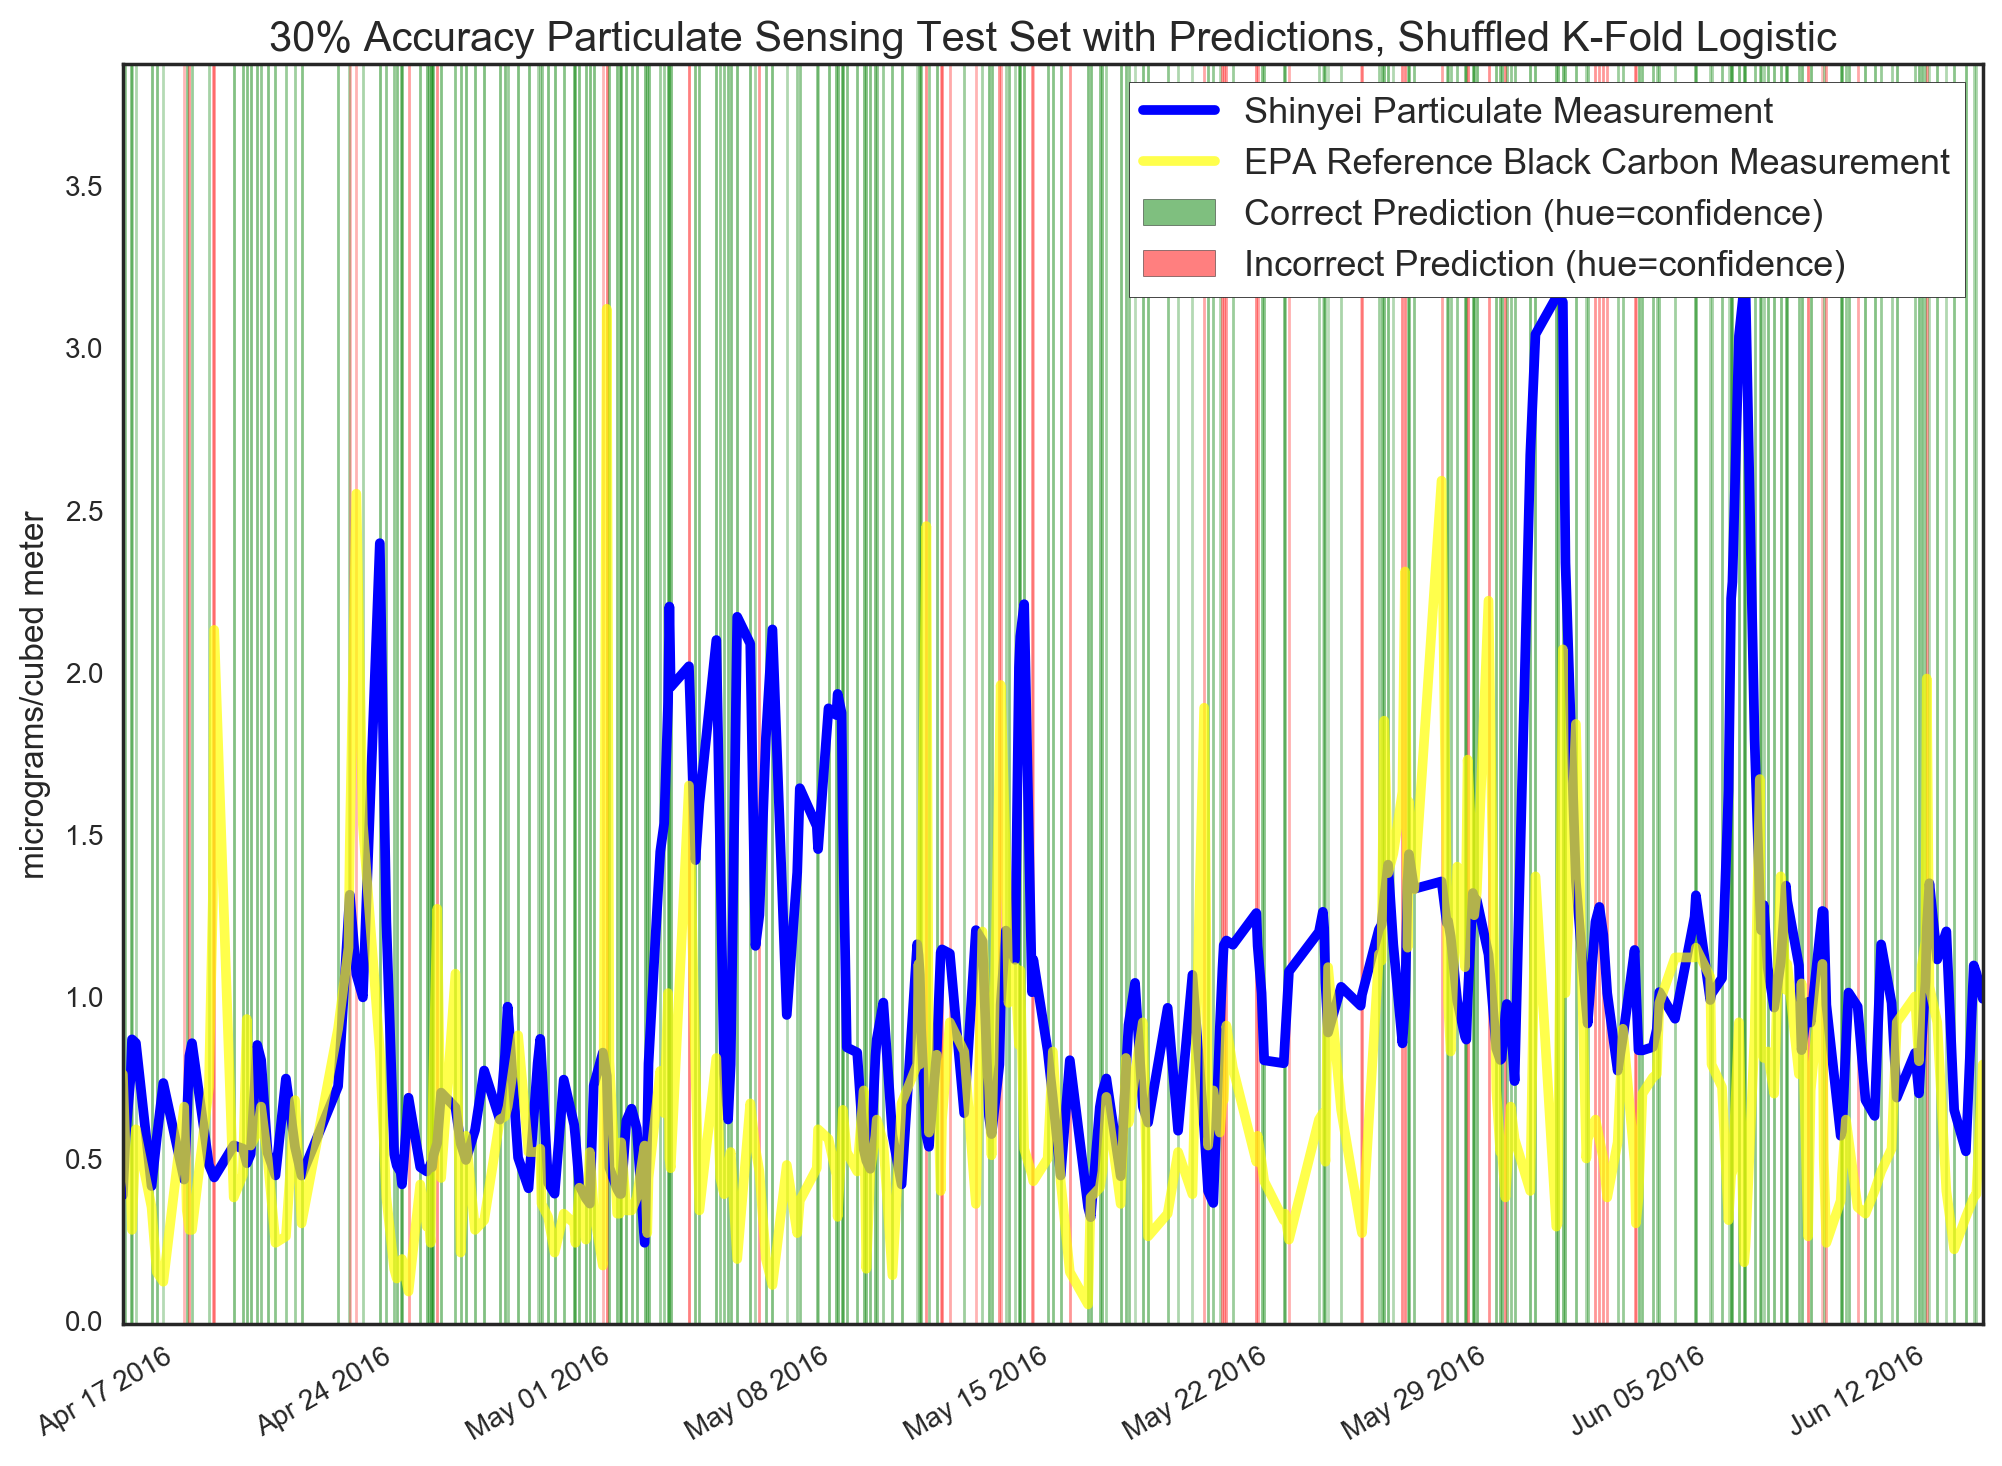
\includegraphics[width=\textwidth]{figs/sharp_goals_30_logistic_predictions}               
 	 \caption{Sharp Particulate Prediction Accuracy}
  	\label{fig:sharp_30_logistic_predictions}
\end{figure}



here's text referencing the (Table \ref{tab:sharp_top_features}).

\begin{table}[H]
\centering
\begin{tabular}{lllllllll}
\\
\\
\toprule
     & Corr. & Lasso & Lin Reg & RF   & RFE  & Ridge & Stability & Mean \\
\midrule
sharpDust                                    & 1     & 0.65       & 0    & 1    & 0.81  & 0.03      & 1    & 0.64 \\
lmse\_scaled\_sharpDust                      & 1     & 0          & 0.03 & 0.65 & 0.83  & 0         & 0.98 & 0.5  \\
scaled\_sharpDust                            & 1     & 0          & 0.02 & 0.65 & 0.83  & 0         & 0.91 & 0.49 \\
avg\_12\_scaled\_sharpDust                   & 0.88  & 0          & 0    & 0.06 & 0.49  & 0.77      & 0.55 & 0.39 \\
derivative\_lmse\_avg\_15\_as\_no2           & 0     & 0          & 0.99 & 0    & 0.97  & 0.15      & 0.02 & 0.3  \\
derivative\_avg\_15\_lmse\_as\_no2           & 0     & 0          & 1    & 0    & 0.97  & 0.15      & 0.01 & 0.3  \\
derivative\_avg\_48\_scaled\_sharpDust       & 0.01  & 0          & 0.99 & 0.01 & 1     & 0.01      & 0    & 0.29 \\
derivative\_lmse\_avg\_48\_scaled\_sharpDust & 0.01  & 0          & 0.89 & 0.03 & 1     & 0.01      & 0    & 0.28 \\
temp\_as\_box\_differential                  & 0.01  & 1          & 0    & 0.22 & 0.47  & 0.13      & 0.05 & 0.27 \\
sck\_humidity\_saturated                     & 0.11  & 0          & 0    & 0    & 0.61  & 1         & 0.01 & 0.25 \\
Nitrogen Dioxide ( kOhm)                     & 0.18  & 0.06       & 0    & 0.02 & 0.72  & 0         & 0.67 & 0.24 \\
daily\_avg\_sck\_humidity                    & 0.24  & 0          & 0    & 0.05 & 0.6   & 0.69      & 0    & 0.23 \\
lmse\_sck\_no2                               & 0.18  & 0          & 0    & 0.02 & 0.72  & 0         & 0.67 & 0.23 \\
avg\_48\_scaled\_sharpDust                   & 0.45  & 0          & 0.02 & 0.01 & 0.88  & 0.18      & 0.07 & 0.23 \\
lmse\_avg\_48\_scaled\_sharpDust             & 0.45  & 0          & 0.02 & 0.01 & 0.87  & 0.2       & 0.06 & 0.23 \\
forecastio\_wind                             & 0     & 0          & 0    & 0    & 0.96  & 0.58      & 0    & 0.22 \\
derivative\_as\_no2                          & 0     & 0          & 0    & 0    & 0.99  & 0.57      & 0    & 0.22 \\
o3                                           & 0.1   & 0.25       & 0    & 0.06 & 0.14  & 0.01      & 0.85 & 0.2  \\
derivative\_Carbon Monxide ( kOhm)           & 0     & 0          & 0.36 & 0.03 & 0.99  & 0.01      & 0    & 0.2  \\
derivative\_lmse\_sck\_no2                   & 0     & 0          & 0.45 & 0.01 & 0.86  & 0         & 0    & 0.19 \\
derivative\_lmse\_sck\_co                    & 0     & 0          & 0.31 & 0.02 & 0.98  & 0.01      & 0    & 0.19 \\
daily\_avg\_forecastio\_humidity             & 0.29  & 0          & 0    & 0.02 & 0.46  & 0.41      & 0.05 & 0.18 \\
forecastio\_rain                             & 0.08  & 0          & 0    & 0    & 0.92  & 0.18      & 0    & 0.17 \\
alphaTemp                                    & 0     & 0          & 0    & 0.01 & 0.75  & 0.39      & 0    & 0.16 \\
\bottomrule
\end{tabular}
\label{tab:sharp_top_features}
\caption{Top Features for Predicting Sharp Particulate}
\end{table}

End Text for Sharp Section.
